\section{ХОД РАБОТЫ}

\subsection{Постановка задачи}

Некоторые изделия проходят контроль качества.
Поток изделий можно считать пуассоновским; средний интервал времени
между изделиями составляет 20 минут. 
Примерно 20\% от общего количества изделий составляют изделия типа И1,
50\% --- И2, 30\% --- И3.
На участке работают два контролёра.

Изделие направляется к свободному контролёру, а если оба контролёра заняты
--- то к тому, у которого меньше изделий, ожидающих обработки.
Контроль одного изделия занимает в среднем 15 минут
(экспоненциальная случайная величина).

По результатам контроля в среднем 5\% изделий бракуются. После контроля
годные изделия подаются на упаковочную машину. Длительность упаковки
одного изделия распределена по гауссовскому закону;
характеристики времени упаковки следующие указаны в
таблице~\ref{tbl:source_data}.

\begin{table}[h!]
  \caption{Характеристики времени упаковки изделий}
  \label{tbl:source_data}
  \centering
  \begin{tabular}{| p{0.2\textwidth} | p{0.35\textwidth} | p{0.35\textwidth} |}
    \hline
    Тип изделия &
    Среднее время \newline упаковки, мин &
    Среднеквадратическое \newline отклонение, мин \\
    \hline
    И1 & 5 & 0{,}5 \\
    \hline
    И2 & 10 & 1 \\
    \hline
    И3 & 15 & 1 \\
    \hline
    \end{tabular}
\end{table}

Требуется разработать GPSS-модель, имитирующую работу участка контроля и
упаковки в течение 48 часов.
Предусмотреть подсчёт количества годных и бракованных изделий каждого типа.

\subsection{Решение задачи}

Разработанная GPSS-модель представлена в приложении~А. После выполнения сеанса
моделирования исходной задачи, получим отчёт, представленные на
рисунках~\ref{pic:report_1}~-~\ref{pic:report_3}.

\begin{figure}[h!]
  \centering
  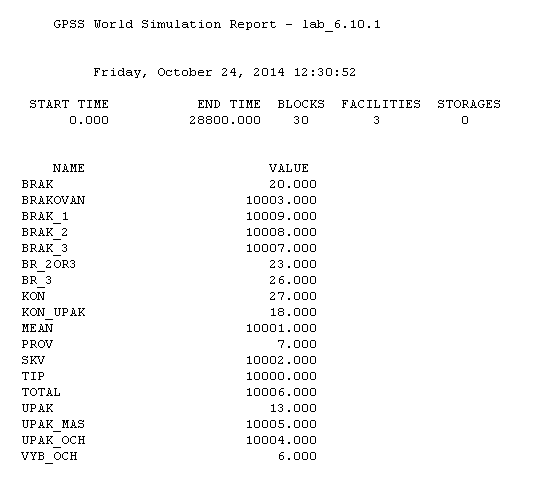
\includegraphics[width=0.75\linewidth]{pic/report_1}
  \caption{Выходные данные имитационной модели}
  \label{pic:report_1}
\end{figure}

\begin{figure}[h!]
  \centering
  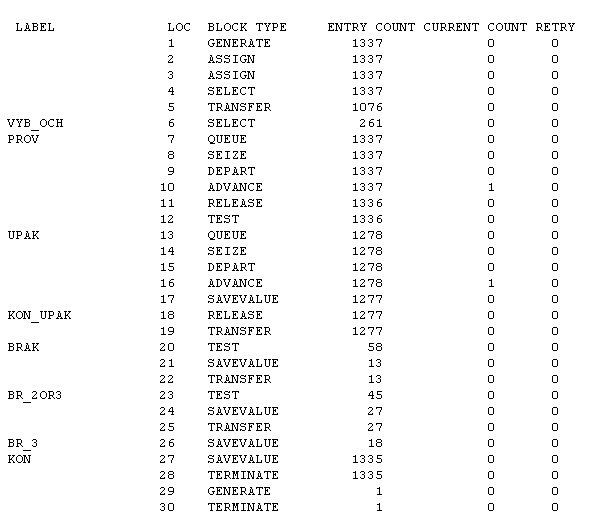
\includegraphics[width=0.75\linewidth]{pic/report_2}
  \caption{Статистика исполнения команд имитационной модели}
  \label{pic:report_2}
\end{figure}

\newpage

\begin{figure}[h!]
  \centering
  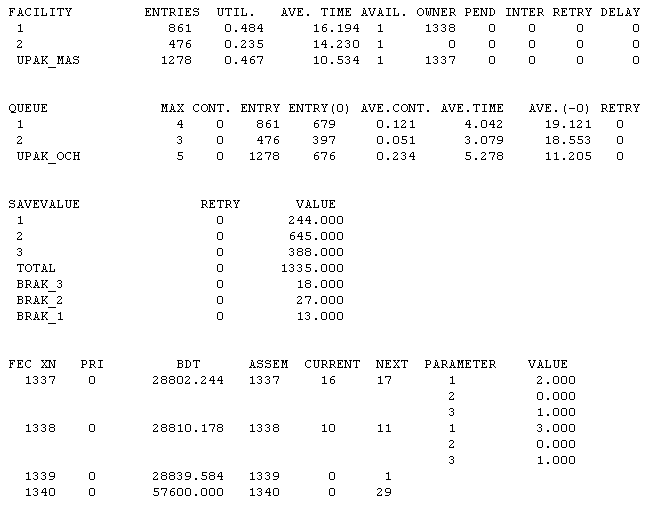
\includegraphics[width=0.9\linewidth]{pic/report_3}
  \caption{Статистика использования узлов имитируемой СМО}
  \label{pic:report_3}
\end{figure}

\newpage
